\section*{Aufgabe 2: Profiling zur Untersuchung eines Algorithmus}

\subsection*{b)}

  \begin{figure}
    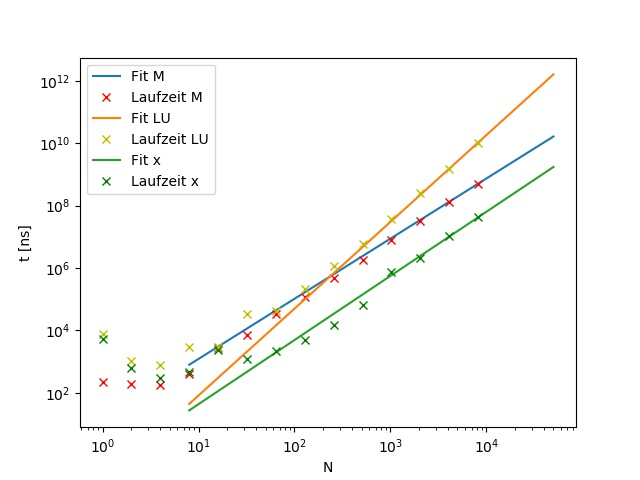
\includegraphics{../../Blatt2/Plots/plot2.pdf}
    \caption{Laufzeiten für das Erstellen der Matrix M, die LU-Zerlegung und das Lösen des Gleichungssystems in Abhängigkeit von N.}
    \label{fig:A2}
  \end{figure}

  \noindent Die in der Abbildung \ref{fig:A2} dargestellten Fits wurden mit der Funktion
  \begin{equation}
    f(x)=a x^b
  \end{equation}
  gefittet. Dabei ergeben sich die Parameter für die Erstellung einer random $N$x$N$ Matrix

  $$a_M = (12.27 \pm 1.4) \text{s}$$
  $$b_M = 1.947 \pm 0.013 ,$$
  für die LU-Zerlegung dieser Matrix
  $$a_{LU} = (0.128 \pm 0.007) \text{s}$$
  $$b_{LU} = 2.789 \pm 0.006$$
  und das Lösen
  $$a_x = (0.4 \pm 0.07) \text{s}$$
  $$b_x = 2.049 \pm 0.019.$$
  Dies sind natürlich nur die zu der Abbildung gehörenden Werte. Bei erneutem Durchlauf des Programmes
  können die Ergebnisse leicht von diesen Abweichen. Zu erkennen ist, dass die Werte erst ab höheren $N$
  auf der Ausgleichsgeraden liegen, für kleinere $N$ liegen sie über den Fits, daher wurden auch diese
  Werte nicht im Fit berücksichtigt.

  \subsection*{c)}

    \noindent i) Gesammtlaufzeit

    \noindent Mithilfe der Ausgleichsgeraden lässt sich abschätzen, dass für $N=1000000$
    die Laufzeit ca bei
    $$t= 6982302.46 \text{s} =  1939.53 \text{h} = 80.81 \text{d}= 0.22 \text{a}$$
    liegt.
    \noindent ii) Optimierungspotential

    \noindent Die LU-Zerlegung hat das größte $b$, mit höheren $N$ steigt die Laufzeit für die Zerlegung
    also stärker an als die für das Erstellen der Matrix und das Lösen der Gleichung. Daher
    würde es sich am meisten auszahlen, die LU-Zerlegung zu optimieren.


  \subsection*{d)}

    \noindent Je größer die Matrix ist, desto mehr Schritte werden benötigt, um Eigenwerte zu berechnen. Daher
    werden auch Rundungsfehler immer größer, sodass die Eigenwerte bei zu großen $N$ nicht mehr vernünftig bestimmt
    werden können.
